\documentclass[5p]{elsarticle}

\usepackage{lineno,hyperref}
\modulolinenumbers[5]

\journal{Journal of \LaTeX\ Templates}

\usepackage{amsmath,amssymb,amsthm}
\usepackage{commath}

\usepackage{graphicx} % Required for including images
\graphicspath{{Figures/}} % Set the default folder for images
\usepackage{glossaries} % Abbreviations
\newglossaryentry{HAR}{
	name={HAR},
	description={Human Activity Recognition}
}

\newglossaryentry{DTC}{
	name={DTC},
	description={Decision Tree Classifier, uses a decision tree as a predictive model}
}

\newglossaryentry{DFT}{
	name={DFT},
	description={Discrete Fourier Transform}
}


\newglossaryentry{RFC}{
	name={RFC},
	description={Random Forest Classifier, uses a ensemble learning method for classification}
}

\newglossaryentry{SVM}{
	name={SVM},
	description={Support Vector Machine, constructs hyperplanes to separate labeled vectors}
}

\newglossaryentry{RBF}{
	name={RBF},
	description={Radial basis function, a real-valued function used as a kernel for multi-class \gls{SVM}}
}

\newglossaryentry{IMU}{
	name={IMU},
	description={Inertial Measurement Unit}
}


%%%%%%%%%%%%%%%%%%%%%%%
%% Elsevier bibliography styles
%%%%%%%%%%%%%%%%%%%%%%%
%% To change the style, put a % in front of the second line of the current style and
%% remove the % from the second line of the style you would like to use.
%%%%%%%%%%%%%%%%%%%%%%%

%% Numbered
%\bibliographystyle{model1-num-names}

%% Numbered without titles
%\bibliographystyle{model1a-num-names}

%% Harvard
\bibliographystyle{model2-names.bst}\biboptions{authoryear}

%% Vancouver numbered
%\usepackage{numcompress}\bibliographystyle{model3-num-names}

%% Vancouver name/year
%\usepackage{numcompress}\bibliographystyle{model4-names}\biboptions{authoryear}

%% APA style
%\bibliographystyle{model5-names}\biboptions{authoryear}

%% AMA style
%\usepackage{numcompress}\bibliographystyle{model6-num-names}

%% `Elsevier LaTeX' style
\bibliographystyle{elsarticle-num}
%%%%%%%%%%%%%%%%%%%%%%%

\begin{document}

\begin{frontmatter}

\title{Human Physical Activity Recognition from Acceleration Data under Naturalistic Conditions}

%% Group authors per affiliation:

\author[dic]{Abhijeet~Parmar\corref{cor1}}
\ead{abhijeet@ducic.ac.in}
\address[dic]{Design Innovation Centre, University of Delhi, Delhi, India 110007}
\cortext[cor1]{Corresponding author}

\author[cic]{Prashant~Sinha}
\ead{prashant@ducic.ac.in}
\address[cic]{Cluster Innovation Centre, University of Delhi, Delhi, India 110007}

\begin{abstract}
Providing accurate and opportune information on people’s activities and behaviors is one of the most important tasks in pervasive computing. Innumerable applications can be visualized, for instance, in medical, security, entertainment, and tactical scenarios. In this study, we explore the detection of human activities (walk, run, jog, climb stairs up, climb stairs down, stand still, biking) from data acquired using single tri-axial accelerometer. We address the task of detecting activities irrespective of the user specific sensor position, orientation and body attachment. We compare the classification accuracies in case of orientation uncorrected data in different positions and orientations across multiple individuals. Also, we show that a single device and accelerometer data is sufficient to detect the activities. Additionally we also show significant activity detection accuracies when the user holds the device in the hand or carries it in the pockets, as in a real life scenario. Random Forest classifiers showed the best performance recognizing everyday activities with an overall accuracy rate of $96\%$. Finally, we present some open problems and ideas that, due to their high relevance, should be addressed in future research.
\end{abstract}

\begin{keyword}
Human Activity Recognition\sep Feature Extraction\sep Windowing\sep Pervasive Computing\sep Random Forest
\end{keyword}

\end{frontmatter}

\linenumbers

\section{Introduction}

Providing and predicting information about user's intent, behaviour, and activities is one of the most important task in pervasive computing. Human Activity Recognition (\gls{HAR}) is a problem of inferring the state of the user by exploiting the data obtained from sensors that are already present in many mobile devices. The information provided from \gls{HAR} system can be utilised to provide contextual awareness which can further be utilised in innumerable applications. Context aware mobile apps may optimize their user experience based on the activity that the user is presently performing. It can also be used in various patient and baby monitoring systems to provide accurate and realtime activity data which may prove useful to the caretakers in case of emergencies \cite{Anguita2013}. Activity information may also be used to remove false positives from pedometer data in fitness tracking applications for more accurate gait analysis.

\section{Previous Work}

Various studies have shown efficiency of machine learning methods for the solution of \gls{HAR} task. \cite{Anguita2013} proposes an energy efficient method of activity classification using fixed point arithmetic scheme for training a \gls{SVM}. The classification accuracy of their scheme is 89\% for 6 activity classes. \cite{Gupta2014} is the closest to the present study. They take a 6 seconds window to compute the features. The method involves further windowing to calculate the features such as mean trends and windowed mean difference. Their result had an accuracy of 97-98\% using kNN and Naive Bayes classifier.

\cite{Banos2014} investigate the relation between window length and the classification accuracy, while \cite{Reyes-Ortiz2015} report success using signal processing and filters on the combined gyroscope and accelerometer data.

\cite{He2009} use PCA and Cosine transform for the \gls{HAR} task. They report 97\% accuracy between 4 activity classes. \cite{Shoaib2013} also use gyroscope and accelerometer data in their study while claiming the decrease in classification accuracy due to the bias arising by shifting the position of the device.

\section{Undertaken Challenge}

\subsection{Hardware Complexity Constraint}
It is required that the task is solved solely through the data from a single triaxial accelerometer. This reduces the hardware complexity.

\subsection{Attitude Independent Recognition (Axis Constraint)}
\label{axis_constraint}
It is required that the task be solved without any prior knowledge of the location and orientation of the motion tracker. This follows from the fact that the motion tracker could be placed at any spot on the user, for example their pockets, their arm or in their hand.

\subsection{Hardware Friendly Classification (Time Complexity Constraint)}
\label{time_constraint}
It is required that the features that are generated from the sensor sample sequence must be computationally low cost. This is required for energy efficient implementation of the technique in various portable devices such as a fitness tracker or a mobile phone.

\section{Method}

\begin{figure}[h!]
  \begin{center}
    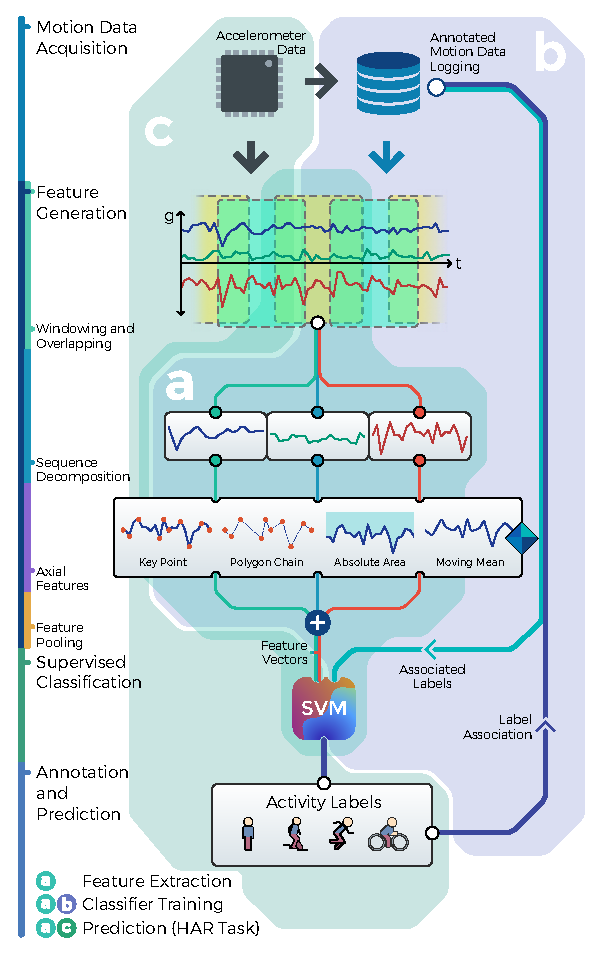
\includegraphics[width=0.5\textwidth]{HAR_Illustration}
  \end{center}
  \vspace{-10pt}
  \caption{\label{har_illustration}Methodology Overview}
\end{figure}

The task of human activity recognition (HAR) begins with data collection. However, the raw data in itself is not representative enough to be used for carrying out the task of classification. Thus, we need to prepare the data by cleaning it and carrying out various data preprocessing activities. The preprocessed data still doesn’t capture the temporal nature of the task. Hence data segmentation is performed to enhance the discriminative power of the data. Feature extraction, then, converts the signals into the most relevant and powerful features which are unique for the activity at hand (Figure \ref{har_illustration}). Finally classification algorithms can be trained on the refined data, and a reliable prediction model can be created

\subsection{Acquisition of Activity Dataset}
Motion data was logged through motion tracking device and an iPhone app developed for the purpose at the sampling rate of 50 Hz while multiple human subjects performed various activities as mentioned in section \ref{activity_classes}. The location of the devices and the duration of activities were neither controlled nor taken into consideration. The subjects were also allowed to move or use the devices during the activity. These events were also not controlled and did not have any exclusive label. This was done to ensure that the dataset reflected the real-world usage pattern. The starting and ending timestamp of the activities were used to label the logged data.

We also obtained the public dataset \cite{Reyes-Ortiz2015} and \cite{Shoaib2014} to further increase the volume of our data. Only the accelerometer data was utilised from the obtained dataset.

\subsection{Activity Classes}
\label{activity_classes}
We define following activity classes to set the scope of the HAR task.
\begin{enumerate}
	\item Stationary
	\begin{enumerate}
		\item Sitting
		\item Standing
	\end{enumerate}
	\item Active
	\begin{enumerate}
		\item Walking
		\begin{enumerate}
			\item Typical
			\item Stair
			\begin{enumerate}
				\item Walking Upstairs
				\item Walking Downstairs
			\end{enumerate}
		\end{enumerate}
		\item Running
		\begin{enumerate}
			\item Typical
			\item Jogging
		\end{enumerate}
		\item Biking
	\end{enumerate}
\end{enumerate}

\subsection{Windowing and Overlapping}
Due to the nature of task, it is often very difficult to represent a particular activity solely through one sample point. Hence, it is recommended to utilise a sequence of signal samples to represent the activity instances \cite{Banos2014}.

In the obtained discrete-time sample sequence, we defined a window of length having $l$ samples for all the three axes as activity instance. The windows were also overlapped to reduce any segmentation bias. The value of $l$, and its effect on classification accuracy is discussed in section \ref{results}.

\subsection{Feature Engineering}
To reduce the computational complexity and enhance the recognition characteristics, feature generation is required. Overall 5 features were calculated for each axis. To conform to the axis constraints as defined in section \ref{axis_constraint}, the features from the three axes were combined to get a final feature vector.

To address the time complexity constraint as defined in section \ref{time_constraint}, all the features are calculated in time domain, since the frequency domain conversion using discrete Fourier transform (\gls{DFT}) is a computationally intensive process.

From the figure \ref{example_activity_instance} it can be observed that various activities are inherently periodic in nature. The features are calculated for all the three axes of the activity instances obtained after windowing and overlapping the data.

\begin{figure}[h!]
  \begin{center}
    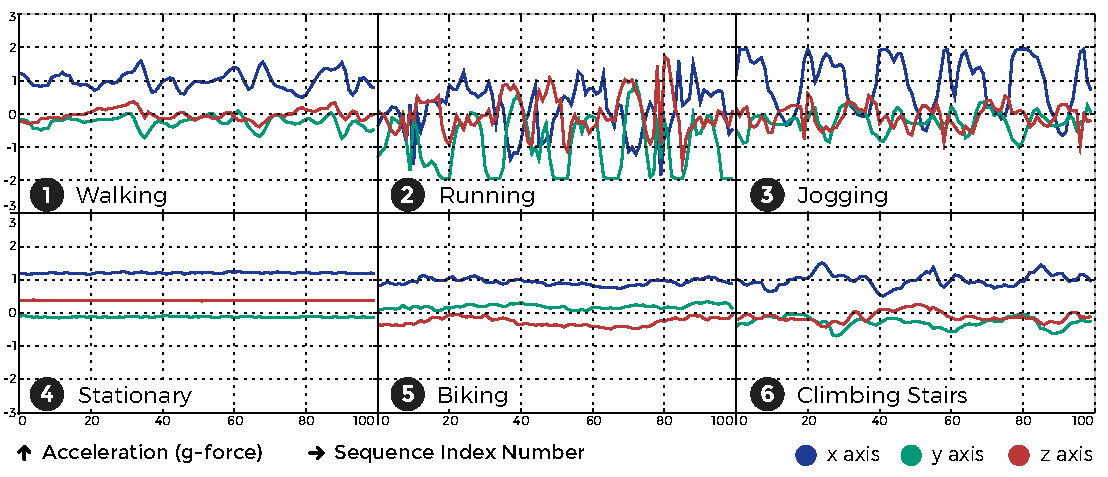
\includegraphics[width=0.5\textwidth]{example_activity_instance}
  \end{center}
  \vspace{-10pt}
  \caption{\label{example_activity_instance}Example instance frames for various activities}
\end{figure}


\subsection{Axial Features}
\label{axial_feature}
Mathematically, the activity instance can be represented by a subsequence of discrete acceleration sample sequence.

Let $S_{raw}$ be a sequence of ordered discrete-time acceleration sample sequence as obtained from the motion tracker. Here, 

\begin{equation} \label{eq:s_raw}
S_{raw}=(\langle a^x_t,a^y_t,a^z_t \rangle)
\end{equation}

where $a^x_t$, $a^y_t$ and $a^z_t$ represent the accelerometer reading at instance $t$, in $x$, $y$ and $z$ axis respectively.

We define the activity instance $S_{act}$ as the subsequence of $S_{raw}$ having length $l$. From $S_{act}$, we further define decomposed axial discrete-time sample sequence by equation \ref{eq:skact}, and indexed sequence by \ref{eq:skrmp}.

\begin{equation} \label{eq:skact}
S^k_{act}=(a^k_i)
\end{equation}


\begin{equation} \label{eq:skrmp}
S^k_{rmp}=(\langle i, a^k_i \rangle)
\end{equation}


where $k\in\langle x, y, z \rangle $ and $i$ is the sequence index.

The axial feature vector is defined in the equation \ref{eq:fk}.

\begin{equation} \label{eq:fk}
F^k = \langle a_{auc}^k, a_{tss}^k, a_{kp}^k, a_{binnedkp}^k, a_{sm}^k \rangle
\end{equation}


The feature vector components are discussed below.

\paragraph{Absolute area under linearly interpolated curve}

Let $f^l_{[i,j]}$ denote the two-point form of a straight line segment joining arbitrary elements in $S^k_{rmp}$. Here,

\begin{equation} \label{eq:fl_ij}
f^l_{[i,j]}=(\frac{a^k_j-a^k_i}{j-i}(x-i)+a^k_j) \quad x \in [i, j)
\end{equation}


We may obtain the linearly interpolated curve function $f_{int}$ as a piecewise function of multiple line segments \cite{Bradie} , defined by$f^l_{[i,j]}$. Hence, if $l$ denotes the number of elements in sequence $S^k_{rmp}$, we get equation \ref{eq:fintk}.

\begin{equation} \label{eq:fintk}
f_{int}^k = (f^l_{[i,i+1]})_{i=0}^{l-1}
\end{equation}


We take the absolute area under $f_{int}^k$ as a feature, which is given by equation \ref{eq:a_auc}

\begin{equation} \label{eq:a_auc}
a_{auc}^k=\int_0^l |f_{int}^k| dx
\end{equation}


\paragraph{Total sum of squares}
Let $\bar{a}^k$ denote the mean of $S^k_{act}$. Then, we obtain the total sum of square for series $S^k_{act}$ as:

\begin{equation} \label{eq:a_tss}
a_{tss}^k = \sum_{n=0}^{l}(a^k_n - \bar{a}^k)^2 \quad \forall a^k_n \in S^k_{act}
\end{equation}

The quantity obtained from equation \ref{eq:a_tss} is used as a feature.

\paragraph{Key point}

We define the key points, $S^k_{kp}$, a subsequence of $S^k_{rmp}$, where the signal sequence attains relative maximum or minimum value (extrema values).

Due to noisy nature of the signal, the relative extrema are estimated by taking $n$ neighbours of the element currently in consideration. The quantity $n$ is defined as the 'order' of extrema function. This is done to ensure that small fluctuations are not accounted as key points.

\begin{figure}[h!]
  \begin{center}
    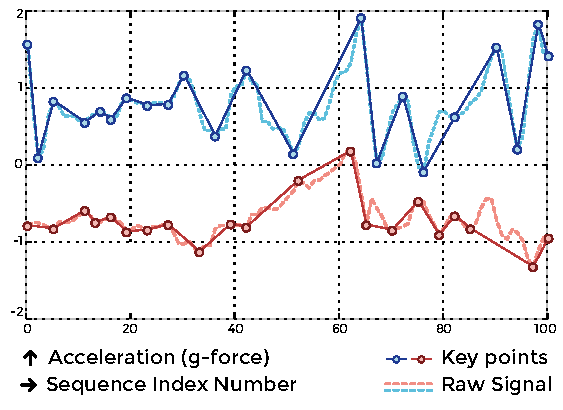
\includegraphics[width=0.45\textwidth]{keypoint_feature}
  \end{center}
  \vspace{-10pt}
  \caption{\label{keypoint_feature}Sample key points selected from raw signal.}
  \vspace{-10pt}
\end{figure}

\paragraph{Key point gradient}
Let

\begin{equation} \label{eq:gk_kp}
G^k_{kp} = (\frac{a^k_j-a^k_i}{j-i})_{i,j}
\end{equation}


be a sequence defined from all consecutive elements $i$ and $j$ in key point sequence $S^k_{kp}$. Here, the elements of sequence $G^k_{kp}$ denote the gradient of a straight line joining the key points.

We take the quantity from equation \ref{eq:a_kp} as a feature.

\begin{equation} \label{eq:a_kp}
a_{kp}^k = Var[G^k_{kp}]
\end{equation}


\paragraph{Binned key point gradient}
We define gradient binning as the process of grouping straight lines on the basis of their gradient. The grouping ranges are obtained by dividing the I and IV quadrants (within the domain of $\arctan$) of cartesian plane in, say, $h$ equal segments. The binning ranges are defined by the following sequence:

\begin{equation} \label{eq:gbin}
G_{bin} = (\langle i, \intco{\tan(\frac{\pi}{h}i), \tan(\frac{\pi}{h}(i+1))} \rangle)_{i=\lceil\frac{h}{2}\rceil}^{\lfloor\frac{h}{2}\rfloor} \quad i \in \mathbb{Z}
\end{equation}


The binning function $f_{bin}$ follows from $G_{bin}$ where, the gradients are given index number $i$, if they fall in corresponding range.

Using $f_{bin}$, we define equation \ref{eq:g_k_binnedkp}, where, $a_i$ are the elements in $G^k_{kp}$.

\begin{equation} \label{eq:g_k_binnedkp}
G^k_{binned kp} = (f_{bin}(a_i))
\end{equation}


We take the following quantity as a feature:

\begin{equation} \label{eq:a_bin_kp}
a_{binnedkp}^k = Var[G^k_{binned kp}]
\end{equation}


\paragraph{Variance of smoothened series}
We use a simple rolling average on $S^k_{act}$ to smooth out the short-term fluctuations in the sequence. We form a new sequence $S^k_{smooth}$ having length $l-n$, where $l$ is the window length and $n$ is the order of rolling average, from $S^k_{act}$. For the elements $e$ in $S^k_{act}$, we have

\begin{equation} \label{eq:sk_smooth}
S^k_{smooth} = (\frac{e_{m}+e_{m-1}+...+e_{m-(n-1)}}{n})_{m=0}^{l-n}
\end{equation}

The following quantity is taken as a feature.
\begin{equation} \label{eq:sk_smooth}
a_{sm}^k = Var[S^k_{smooth}]
\end{equation}

\subsection{Axial Feature Pooling and Feature Vector}
To conform to the Axis Constraint, as defined in section \ref{axis_constraint}, the axial feature vectors $F^x$, $F^y$, and $F^z$ are combined (pooling) to obtain an axis independent feature vector. The variance features, $ \{a_{kp}^k, a_{binnedkp}^k, a_{sm}^k\} $ are pooled by taking the combined variance. We take arithmetic mean of feature $ \{a_{auc}^k, a_{tss}^k\} $. Here, $k$ denotes the three orthogonal axes $x$, $y$, and $z$ as mentioned in section \ref{axial_feature}.


\subsection{Classification using Supervised Learning}
Various supervised learning schemes were utilised for the motion classification. The classifiers were trained using the labelled feature vectors and the resulting classifier was then used for cross validation and prediction.

\subsection{Realtime Activity Prediction}
To implement the realtime activity classification, the triaxial accelerometer is sampled at a sampling rate of 50 Hz. These samples are stored in a buffer array and then the feature vector is  calculated for this buffer array. The predicted activity label for this feature vector is obtained by fitting the vector into the trained classifiers.

\section{Feature Classification}
\label{feature_classification}

Since the \gls{HAR} task requires that multiple activities are classified, a multi-class classifier is required. We explored various multi-class supervised-learning methods to evaluate the classification performance of the features as discussed in section \ref{axial_feature}. The methods that were evaluated are: Decision Tree Classifier (\gls{DTC}), Random Forest Classifier (\gls{RFC}), and Support Vector Machine (\gls{SVM}) with \gls{RBF} Kernel with varying parameters.

The performance as well as the relevance of the features are discussed in section \ref{results}.

\section{Results and Discussions}
\label{results}
\subsection{Results}

After calculating the features for the windows, and assigning the labels, we split the dataset into two segments with random cuts. First segment, having $75\%$ the size of the dataset, was used for training the classifiers. The other segment, representing the $25\%$ of the dataset, was used for testing purpose. The same data-subset was used for evaluating all the classifiers as mentioned in section \ref{feature_classification}.

Figure \ref{cls_rpt} contains the classification accuracy obtained by each classifier with respect to the chosen window length. Using the dataset as mentioned in section \ref{results}, we obtained a maximum classification accuracy of $96.32\%$ using Random Forest Classifier closely followed by Support Vector Machine with $95.05\%$ accuracy (Figure \ref{cm_fig}).

\begin{figure}[b!]
  \centering
  \begin{center}
    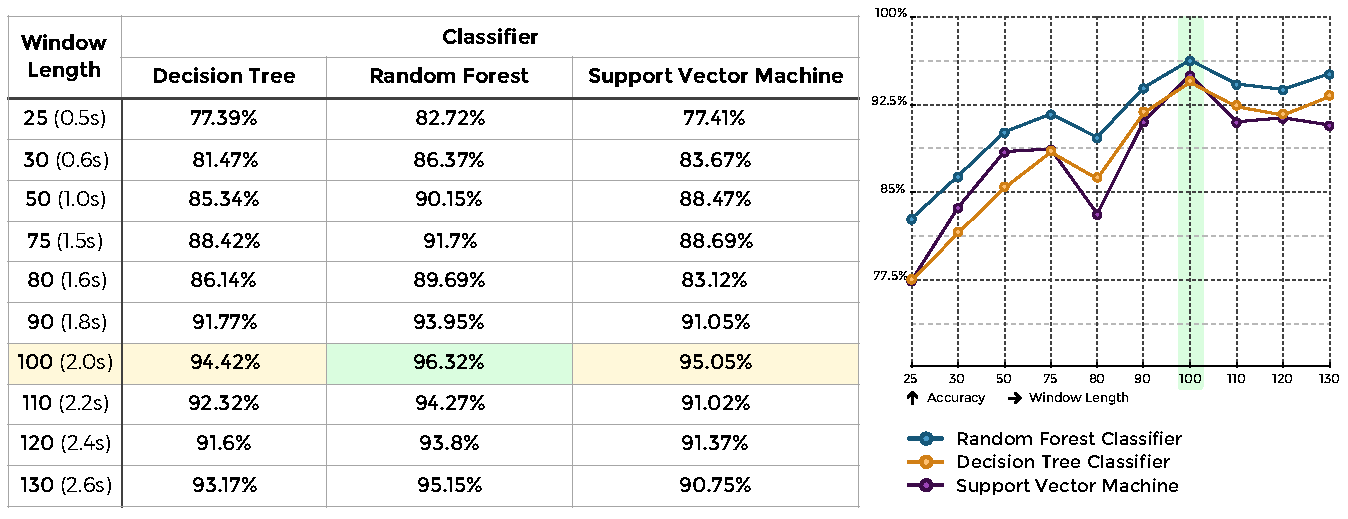
\includegraphics[width=0.5\textwidth]{Classification_Report}
  \end{center}
  \vspace{-10pt}
  \caption{\label{cls_rpt}Comparative classification accuracy for varying window sizes.}
  \vspace{10pt}
\end{figure}

\begin{figure}[h!]
  \centering
  \begin{center}
    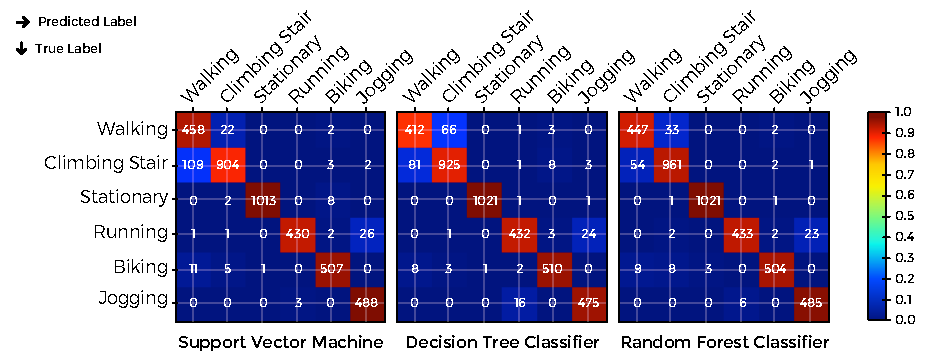
\includegraphics[width=0.5\textwidth]{Confusion_Matrix}
  \end{center}
  \vspace{-10pt}
  \caption{\label{cm_fig}Confusion Matrix for window length $l=100$.}
\end{figure}

\subsection{Discussions}
Human activities are performed during relatively long periods of time compared to the sensors sampling rate. Besides, a single sample on a specific time instant does not provide sufficient information to describe the performed activity. Thus, activities need to be recognized in a time window basis rather than in a sample basis. Now, the question is: how do we compare two given time windows? It would be nearly impossible for the signals to be exactly identical, even if they come from the same subject performing the same activity. This is the main motivation for applying feature extraction methodologies \cite{Guyon2003} \cite{Chen2006} to each time window: filtering relevant information and obtaining quantitative measures that allow signals to be compared.In general, two approaches have been proposed to extract features from time series data: statistical and structural. In our study, we have used a combination of both statistical and structural features.

In addition to efficient feature extraction, selection of window length that is dividing the measured time series in time windows is also crucial in increasing the classification accuracy. A key factor is, therefore, the selection of the window length because the computational complexity of any feature extraction method depends on the number of samples. Having rather short windows may enhance the feature extraction performance, but would entail higher overhead due to the recognition algorithm being triggered more frequently. Besides, short time windows may not provide sufficient information to fully describe the performed activity. Conversely, if the windows are too long, there might be more than one activity within a single time window. Different window lengths have been used in the study but the maximum classification accuracy is observed with window length of 2s. Of course, this decision is conditioned to the activities to be recognized and the measured attributes.

Figure \ref{parallel_plot} is the parallel coordinate visualisation \cite{Wegman1990} of $50$ feature vectors, chosen randomly, for each activity class as described in section \ref{activity_classes}. We used parallel coordinates to plot the components in order as presented in figure. The independence between individual features is clearly distinguished for the activity classes. The feature vectors are plotted in both Linear and Logarithmic scale to improve visibility of features that attain value close to zero, since the features are not normalised.

\begin{figure}[h!]
  \begin{center}
    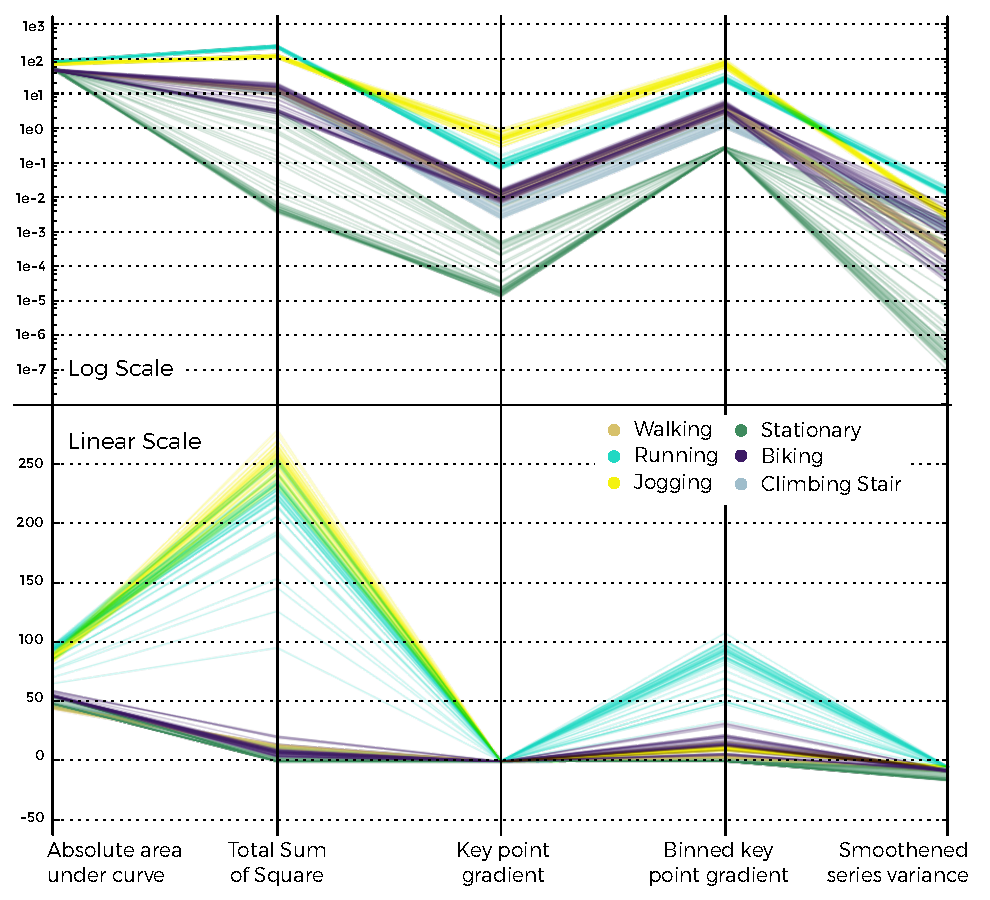
\includegraphics[width=0.5\textwidth]{ParallelPlot}
  \end{center}
  \vspace{-10pt}
  \caption{\label{parallel_plot}Parallel coordinates plot of feature vectors.}
  \vspace{5pt}
\end{figure}


Similarly, figure \ref{radviz_plot} is the RadViz Visualisation \cite{Sharko2008}\cite{Bertini2005} of 400 feature vectors chosen randomly for each activity classes. Distinct clusters of activity classes further support the conclusion made from the Parallel Coordinate plot of feature vector. Confusion between similar activities, such as Jogging and Running, and Walking and Climbing is also visible in the plot wherever the cluster of classes overlap. However, it should be noted here that only a small percentage of feature vectors overlap, as evident from section b in figure \ref{radviz_plot}.

\begin{figure}[h!]
  \begin{center}
    \includegraphics[width=0.48\textwidth]{RadViz}
  \end{center}
  \vspace{-10pt}
  \caption{\label{radviz_plot}RadViz visualisation of feature vectors.}
  \vspace{-10pt}
\end{figure}


\newpage
\section{Conclusion}
The focus of this research was to explore and analyze flexibility in various constraints, specifically the position, orientation and attachment of the mobile sensor device in a human activity recognition task. The results from our study provide evidence to the fact that activity recognition is possible in spite of variation in the aforementioned constraints. Our findings also indicate that neither device orientation information nor orientation correction appear to be necessary, as we are able to correctly classify the activities across all subjects without orientation correction. Moreover, by using simple features, we can achieve high classification accuracies, above 95\% irrespective of how the device is carried and placed by the subject. This method is suitable for a distributed system where users can report data, in real-time or in batches, and this information can be processed and used to act according to the individual context.

The results of the present research have been submitted for publication in International Journal of Human-Computer Studies.


\section*{References}

\bibliography{mybibfile}

\end{document}